\documentclass{article}
\usepackage{amsmath,amsthm,amssymb}
\usepackage{mathtext}
\usepackage[T2A]{fontenc}
\usepackage[utf8]{inputenc}
\usepackage[english]{babel}
\usepackage{graphicx}
\usepackage{hyperref}
\usepackage{mathtools}


\title{STONKS - Stock Market Forecasting Using News Articles With Reinforcement And Sequence Learning}
\author{Ruslan Sirazhetdinov} 

\date{May 2023}



\begin{document}
\maketitle
\begin{abstract}
    I believe, that there is a correlation between price change direction of a particular share and news articles. The purpose of this project is to predict market price for next day, each time depending on news of the current. The project consists of my own StocksNews dataset, the baseline solution, experiments with existing related solutions, implementation of custom Stocks reinforcement learning environment, making of proposed solution using a combination of reinforcement learning and sequence learning techniques.
    \url{https://github.com/irusland/nlpystocks}.
\end{abstract}



\section{Introduction}
Stock market if a highly variable environment and for the its forecasting you need to know how to act in certain situation. 
There is no doubt that stocks market prediction is a highly non linear relation to the news articles. The situation on the market can change drastically in a moments without any prior information because of the insiders policies, non disclosure agreements. But still, there are many cases when a random tweet from Elon Musk could literally heat up the whole investors community.

The news could be a pretty helpful tool for decision making. 
It most likely has a little average impact on the market in general, but news could provide some hints for enhancing the forecasts.

Its important to know these aspects during making a decision to invest or not. This work could be a possible baseline for a more complex trading bot that processes all the big data information in realtime.

Primarily, the approach to forecast the timeseries is to train a particular model, it may be a linear or statistically or neural network based model. Ensembles or a combination of models is also possible. You have some training data, and you validate you model on the data that has not been seen by the model. 

The difference in my approach is that I have tried to use a human-like actions.
The requirements for the model is to make a decision to invest or not, or temporarily suspend any trading.
It's possible with the use of reinforcement learning and building a deep Q-networks.
This differs from the regression solving models, because after getting the model's predictions there are many ways to operate with received data. The naive approach could be hard-coding some instructions based on conditional logic. For example: if the market price goes up and reaches the certain threshold we make a decision to buy shares. 
This is a major flaw of such algorithms in my opinion, and that is why I have chose to mimic real human's actions.

In this work I proposed a sequence learning network architecture and implemented an reinforcement environment for training of such network.

\subsection{Team}
\textbf{Sirazhetdinov Ruslan} \href{mailto:sirazhetdinov.rr@phystech.edu}{sirazhetdinov.rr@phystech.edu}

I was the only one participant in the team and responsible for several goals:

\begin{enumerate}
  \item  determination of current state of the art solutions and related works.
  \item  researching the topic of existing datasets that will suit the need of this work.
  \item  preparation of news and stocks dataset, with custom human-like crawler.
  \item  making a simple baseline solution.
  \item  adapting existing models from related works for dataset.
  \item  developing of custom reinforcement learning environment.
  \item  implementation of proposed solution.
  \item  gathering the results.
  \item  writing a report.
  
\end{enumerate}


\section{Related Work}
\label{sec:related}

In this section I will provide my understanding and implementation of currently available solutions to the forecasting problem

\subsection{Sequence learning using recurrent logic}
A Robust Predictive Model was presented in the paper \cite{Sen_2021}.
The key idea for the prediction is to process not only the current moment of time but also previous data with some kind of lag measured in days.
The authors introduce us to their successful experiment with recurrent neural network. They also show the results of some linear-based models but, they say "stock price movement is a highly non-linear process".

The experiment consists of preparation of the data with some kind of Natural Language Processing, which is unclear to me, how did they manage to get embeddings from sentences. So I chose the TF-IDF embeddings, and min-max scaler for recieved data.

The main model contained LSTM \cite{HochSchm97} module and fully connected layers to predict a single float number - the price.
LSTM (Long Short-Term Memory) is a type of recurrent neural network (RNN). The main advantage of LSTMs over traditional RNNs is their ability to learn and store long-term dependencies in the input sequence. This is achieved through the use of specific memory cells that store information and a set of gates that control access to these memory cells. 
The memory cells and gates allow LSTMs to selectively remember or forget information from the input sequence, which makes them good for tasks that rely on understanding context and long-term dependencies.

I was not able to find a suitable source code for solution, some haven't provided a source code links, and others have been implemented in different programming languages like java, 
Since i am using python as a tool in this research, I have tried to implement my own representation according to experiment notes in papers.

The news were classified into moods such as positive, negative, neutral and one-hot encoded.
The Lag was set to 3, as the best one mentioned in paper so model receives news from 3 previous time points. The hidden size was 42, this parameter controls the number of parameters in the LSTM layer, and thus affects the model's capacity to capture complex patterns and dependencies in the input data.

After implementation and 100 epochs of MSELoss via Adam optimisation algorithm I achieved pretty decent results which will be described in Results\ref{sec:results}

\subsection{Sequence learning using Fuzzy logic}

A Self-Organizing Fuzzy Neural Network is proposed by \cite{SalimiBadr2022}.
SOFNN is a type of artificial neural network that combines the techniques of fuzzy logic and neural networks.
Interestingly enough, this architecture solves the task of unsupervised learning.
It's designed to automatically identify the underlying structure of the data and create fuzzy rules that accurately describe the input-output relationship of the system being modeled. It consists of four layers: input layer, fuzzy layer, normalization layer, and output layer.
The learning process in SOFNN involves the self-organization of the fuzzy rules, which are generated through a clustering process that groups similar data points together and determines the centers of the fuzzy sets. 
These fuzzy rules are then optimized to minimize the error between the network output and the desired output.

While implementing an architecture, for I chose KMeans clusterization algorithm \cite{Hartigan1979} for sequence locator, the module which is responsible for finding the best matching fuzzy rule for a given input pattern with the number of clusters equal to 4. 
For sequence identifier I have used a two layered fully connected network with 100 neuons on each layer.
I have experimented with different optimisers, losses and learning rates, but sadly enough, was not able to get satisfactory results.


\section{Model Description}
The techniques and experiments in related papers got me thinking about combining it with reinforcement learning techniques.
Because reinforcement Learning, is a type of machine learning in which an agent learns how to take actions in an environment in order to maximize a reward.

The environment ---------------------------------

For the agent action space I chose 3 discrete numbers, representing a stages




Here you need to write a detailed description of your approach. It is important to mention that this description should give more details than the descriptions from section \ref{sec:related}\footnote{This is an example of internal references and footnotes at the same time.}. 

You will likely be providing a figure to better present your approach. A sample circle is presented on Fig.~\ref{fig:circle}.

The other possible contents of this section are formulae. They could be on a new line:
$$S=\pi r^2,$$
or they could be inline, e.g. if you want to describe the used variables, like $S$ is an area of a circle, while $r$ is its radius. 

\begin{figure}[!tbh]
    \centering
    
\includegraphics[width=0.3\linewidth]{circle.png}
    \caption{A sample circle.}
    \label{fig:circle}
\end{figure}

\section{Dataset}

For the task of predicting stock market i needed a dataset with news articles and current market state.
I have researched for avalable datasets, and there where plenty of twitter's related ones.
I wanted to experiment on Russian stock market via using Russian news. 
And specifically, i did not chose the existing news datasets because they were too broad on topics. My goal was to process only financial related articles.
So my choice was the Finam's newsline\footnote{Raw content from Finam's newline could be found ~\href{https://www.finam.ru/publications/selection/united/}{here}.} also i was their client.

I should mention that, it was not easy to get it downloaded. 
My first naive approach was to just load it using \href{https://pypi.org/project/requests/}{python requests}. But it turned out that they had an interface, where you need to click on the button in order to load another portion of news. So i discovered \href{https://pypi.org/project/selenium/}{python selenium}, a new approach to emulate human-like gestures and button clicks on the web page.
The notebook \texttt{/notebooks/news-scraping.ipynb} consist of scraping a web page with news.

It is important to mention that the dataset is available for the research purposes. 
Since Finam does allow to use the information with giving a link to in according to \href{https://www.finam.ru/about/copyright/}{copyright policy}
Each row contains HTTP link to the source.

The second stage in the notebook \texttt{/notebooks/stocks-dataset.ipynb} was to load a stock market values from stock exchange. 
As an employee of Tinkoff bank and an active contributor of \href{https://github.com/Tinkoff/invest-python}{invest-python library} i used the Tinkoff Investments OpenAPI \footnote{Tinkoff Invest OpenAPI could be found ~\href{https://www.tinkoff.ru/invest/open-api/}{here}.} to load the Sberbank privileged shares with FIGI number \texttt{BBG0047315Y7} for the period of previous year. I chose the Sberbank shares instrument because it has high liquidity and high volatility. I believe that such instrument is quite popular among investors.

Having two separate datasets, I have joined them together by matching a \texttt{date} column that contained current date. 
See the details in \texttt{notebooks/dataset.ipynb}.

\begin{figure}[!tbh]
    \centering
    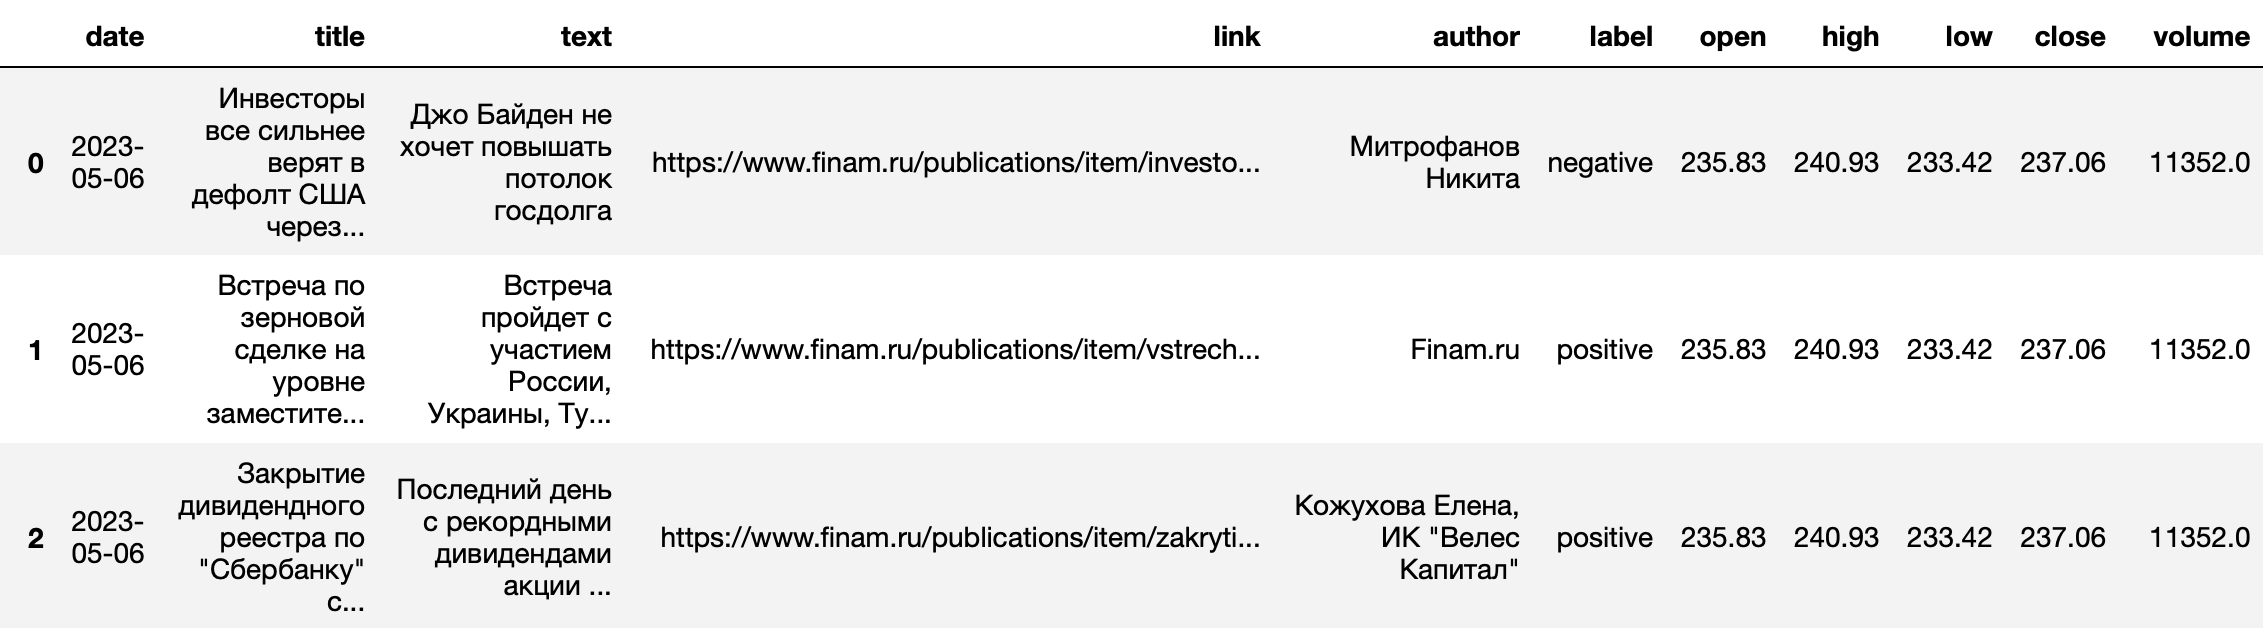
\includegraphics[width=0.9\linewidth]{dataset.png}
    \caption{Dataset samples represented as DataFrame.}
    \label{datased}
\end{figure}

I represent some statistics of resulting StocksNews dataset on Tab.~\ref{tab:statistics} The dataset was split into two parts: train and test with proportion of 88/22 percent accordingy. It's important to mention that this is a time series dataset so I did not use any king of shuffling. 

\begin{table}[tbh!]
\begin{center}
\begin{tabular}[t]{|l|cc|}
\hline
%\cline{2-4}
 & Train & Test \\
\hline
Proportion & 0.88 & 0.22  \\
Size & 23879 & 6735 \\
Vocabulary size & \multicolumn{2}{c|}{16507} \\
Date range & 2022.05.08 - 2023.02.10 & 2023.02.10 - 2023.05.06 \\

\hline
\end{tabular}
\caption{Statistics of the StocksNews dataset.}
\label{tab:statistics}
\end{center}
\end{table}

\begin{figure}[!tbh]
    \centering
    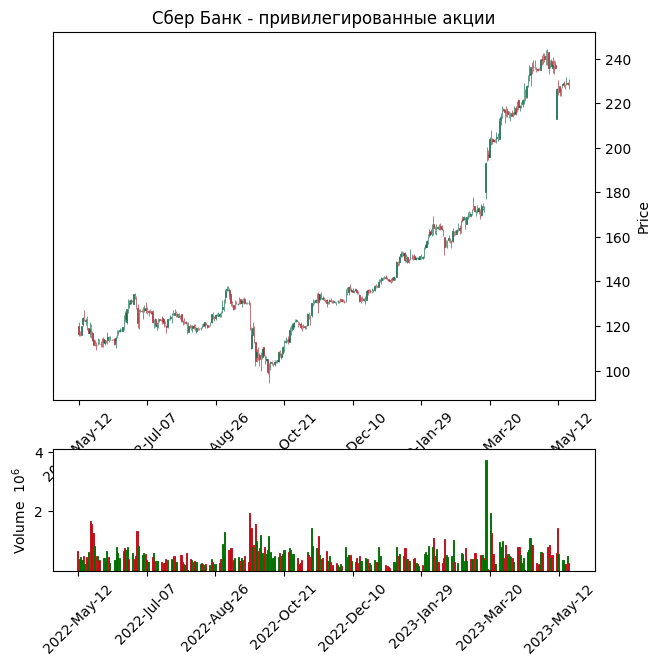
\includegraphics[width=0.9\linewidth]{sber.png}
    \caption{Sberbank shares cost values in dataset.}
    \label{fig:sber}
\end{figure}

When constructing a baseline with TF-IDF\footnote{TF-IDF model to get the sentence embeddings. Details at ~\href{https://ru.wikipedia.org/wiki/TF-IDF}{Wikipedia} or in work by \cite{Ramos1999}.} embeddings, I have used lowercase sentences, \texttt{mystem} for lemmatizaton, \texttt{nltk} for stopwords filtering.

It's worth mentioning that the using the other dataset preprocessing techniques have not been done and could be other possible research topics which is out of scope of current.

For implementing a related work solutions I have labeled every sentence with one of four sentiment labels which was correct in my personal opinion as a novice investor. The distibution of labels is shown of Pic. ~\ref{fig:labels}

\begin{figure}[!tbh]
    \centering
    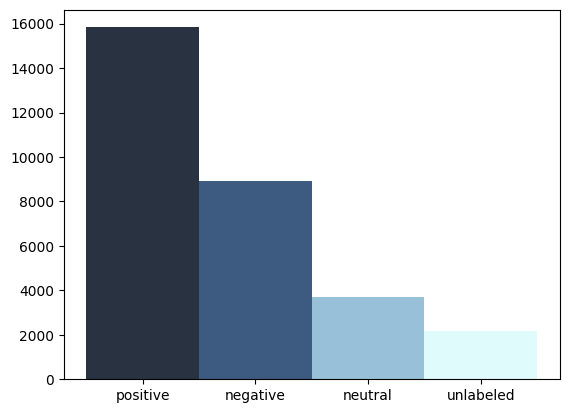
\includegraphics[width=0.5\linewidth]{labels.png}
    \caption{Distribution of sentiment labels in dataset.}
    \label{fig:labels}
\end{figure}



\section{Experiments}
This section should include several subsections.
\subsection{Metrics}
The evaluation of every solution was scored by 2 types of metrics: regression and classification metrics.
My goal was not only to see how close the forecast is to real data via checking regression metrics score, but also to check whether the predictions are correct in the terms of market change direction. And see if you can rely on it during trading.
For that I have used classification metrics.

Following sections contains $\hat{y}$ and $y$ as a forecast values and actual values respectively.

\paragraph{Regression metrics}  

The first is Mean Squared Error:
\begin{align}
MSE(y, \hat{y})=\sum_{i=1}^{D}(y_i-\hat{y}_i)^2,
\end{align}
this metric was chosen to have a general sense of how close the forecasts are.

For intuitive interpretation the Mean Absolute Percentage Error was used:
\begin{align}
{MAPE(y, \hat{y})={\frac {100\%}{n}}\sum _{t=1}^{n}\left|{\frac {y_{t}-\hat{y}_{t}}{y_{t}}}\right|}
\end{align}
\paragraph{Classification metrics}

The accuracy was also used to have a comprehension of models correct choices. I named it as Stock Option Accuracy Score:

\begin{align}
SOAS(y, \hat{y}) = ACC(z, \hat{z}),
\end{align}
\begin{align}
where \quad ACC(z, \hat{z}) = \frac{\left|\{z_i == \hat{z}_i \mid i = 0...n\}\right|}{n}, \nonumber 
\end{align}
 \begin{align}
    where \quad z_{i} = \begin{dcases*}
        1, & if $ y_{i+1} - y_{i} > 0 $,\\
        0, & otherwise. 
        \end{dcases*} \nonumber 
  \end{align}
 \begin{align}
    where \quad \hat{z}_{i} = \begin{dcases*}
        1, & if $ \hat{y}_{i+1} - \hat{y}_{i} > 0 $,\\
        0, & otherwise. 
        \end{dcases*} \nonumber 
  \end{align}


I also came up with a metric Stock Possible Profit Percent Score or S3PS for short:
\begin{align}
S3PS(y, \hat{y}) = 100 * [\prod_{i=0}^{n-1}{(1 + C_i)} - 1],
\end{align}
\begin{align}
where \quad C_i = \begin{dcases*}
        P_i, & if $ y_{i+1} - y_{i} > 0  \quad and \quad \hat{y}_{i+1} - \hat{y}_{i} > 0 $,\\
        P_i, & if $ y_{i+1} - y_{i} <= 0  \quad and \quad \hat{y}_{i+1} - \hat{y}_{i} <= 0 $,\\
        -P_i, & otherwise. 
        \end{dcases*} \nonumber 
\end{align}
\begin{align}
where \quad P_i = \left| 1 - (y_{i+1}/y_{i}) \right| \nonumber 
\end{align}

It is based on SOAS but represents possible percentage gain if we follow a strategy sugested by model.


\subsection{Experiment Setup}
Secondly, you need to describe the design of your experiment, e.g. how many runs there were, how the data split was done. The important details of your model, like hyper-parameters used in the experiments, and so on.

\subsection{Baselines}
Another important feature is that you could provide here the description of some simple approaches for your problem, like logistic regression over TF-IDF embedding for text classification. The baselines are needed is there is no previous art on the problem you are presenting.

\section{Results}
\label{sec:results}

Results for LSTM
Test MSE 0.007547988662526805
Test MAPE 0.07306125655346457
Test SOAS 0.4117647058823529
Test S3PS 4.930981460943817


In this section, you need to list and describe the achieved results. It is crucial to have the results of the experiments for the other approaches. This is needed to be able to compare your results with some competitors. Most preferably, you should provide some references with results on the same problem.

Almost inevitably the results are presented as a table, but it is also possible to have a graph, i.e. a figure.

You need also to provide an interpretation of the presented results, to describe some features. E.g. your approach shows higher results on the short texts or by one metric instead of another.

Also in this section, you could provide some results for your model inference. The samples could be found in Tab.~\ref{tab:output}.

\begin{table}[!tbh]
    \centering
    \begin{tabular}{|c|}
\hline
Это пример вывода вашей модели на русском.\\
This is a sample output of your model in English.
\\
\hline
    \end{tabular}
    \caption{Output samples.}
    \label{tab:output}
\end{table}

\section{Conclusion}
In this section, you need to describe all the work in short: what you have done and what has been achieved. E.g. you have collected a dataset, made a markup for it and developed a model showing the best results compared to other models. 

\bibliographystyle{apalike}
\bibliography{lit}
\end{document}
